There are two variants of interprocedural analysis, context sensitive 
and context insensitive. In context sensitive analysis only interprocedural valid paths are considered during the data-flow
unlike context insensitive in which some invalid paths may also be considered. 

\begin{example}
Consider a program in which {\tt main} function has $2$ call statements for the function {\tt p1}.
Figure~\ref{fig:Some}(a) shows the global control flow graph of both the procedures, which considers
each call statement as a goto from that statement to the start of the called procedure, and 
similarly treats each return statement as goto from that statement to the instruction following
the call statement. For sake of clarity we introduced return blocks after each call statement.

Let the data flow values available just before the call statement {\tt c1} is {\tt df1} and 
that before {\tt c2} is {\tt df2} and they will be entering the function {\tt p1} when called 
at {\tt c1}, {\tt c2} respectively. Similarly, let the corresponding data flow values returned 
from the function {\tt p1} to the statements following {\tt c1} and {\tt c2}
be {\tt df1'} and {\tt df2'} respectively.
If we notice the edges between the functions {\tt main} and {\tt p1}, there is a path {\tt c1}, 
{\tt Enter p1}, {\tt Exit p1}, {\tt return p1} (i.e.\ the block below call-block c2); which is 
not followed in any execution sequence and hence it is not an inter procedurally
valid path. When such paths are considered during data-flow, imprecise data is obtained leading to
imprecise results. Such an analysis is called context insensitive, and the analysis becomes context 
sensitive when we don't consider such invalid paths.
\end{example}

\begin{figure}[h]
\begin{tabular}{c  c}
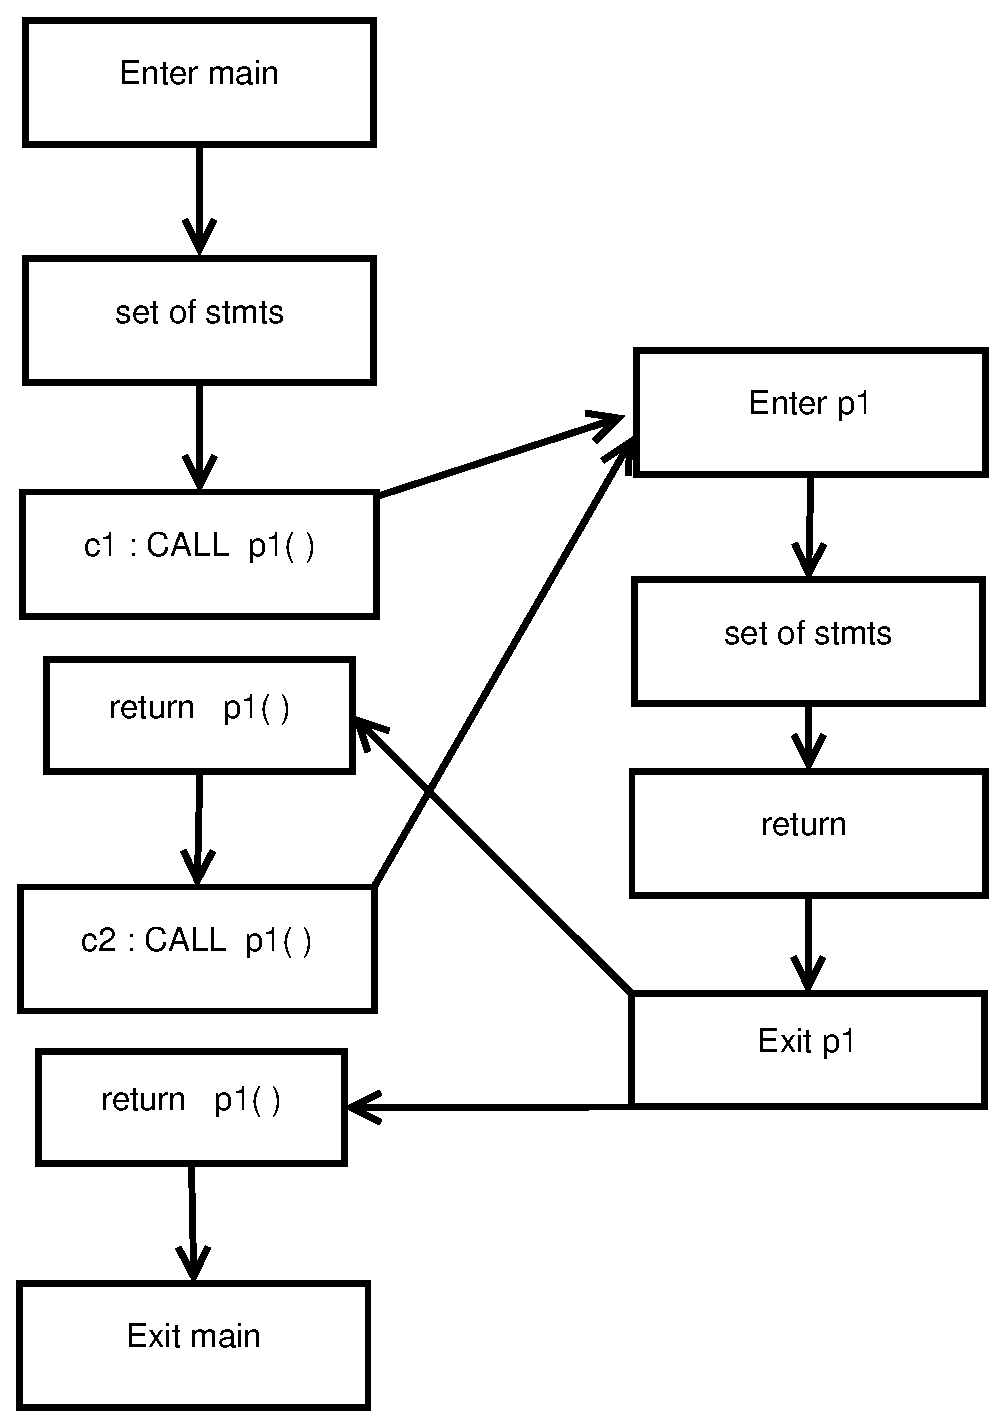
\includegraphics[scale=.23]{Figures/Diagram1.eps} 
& \   \   \
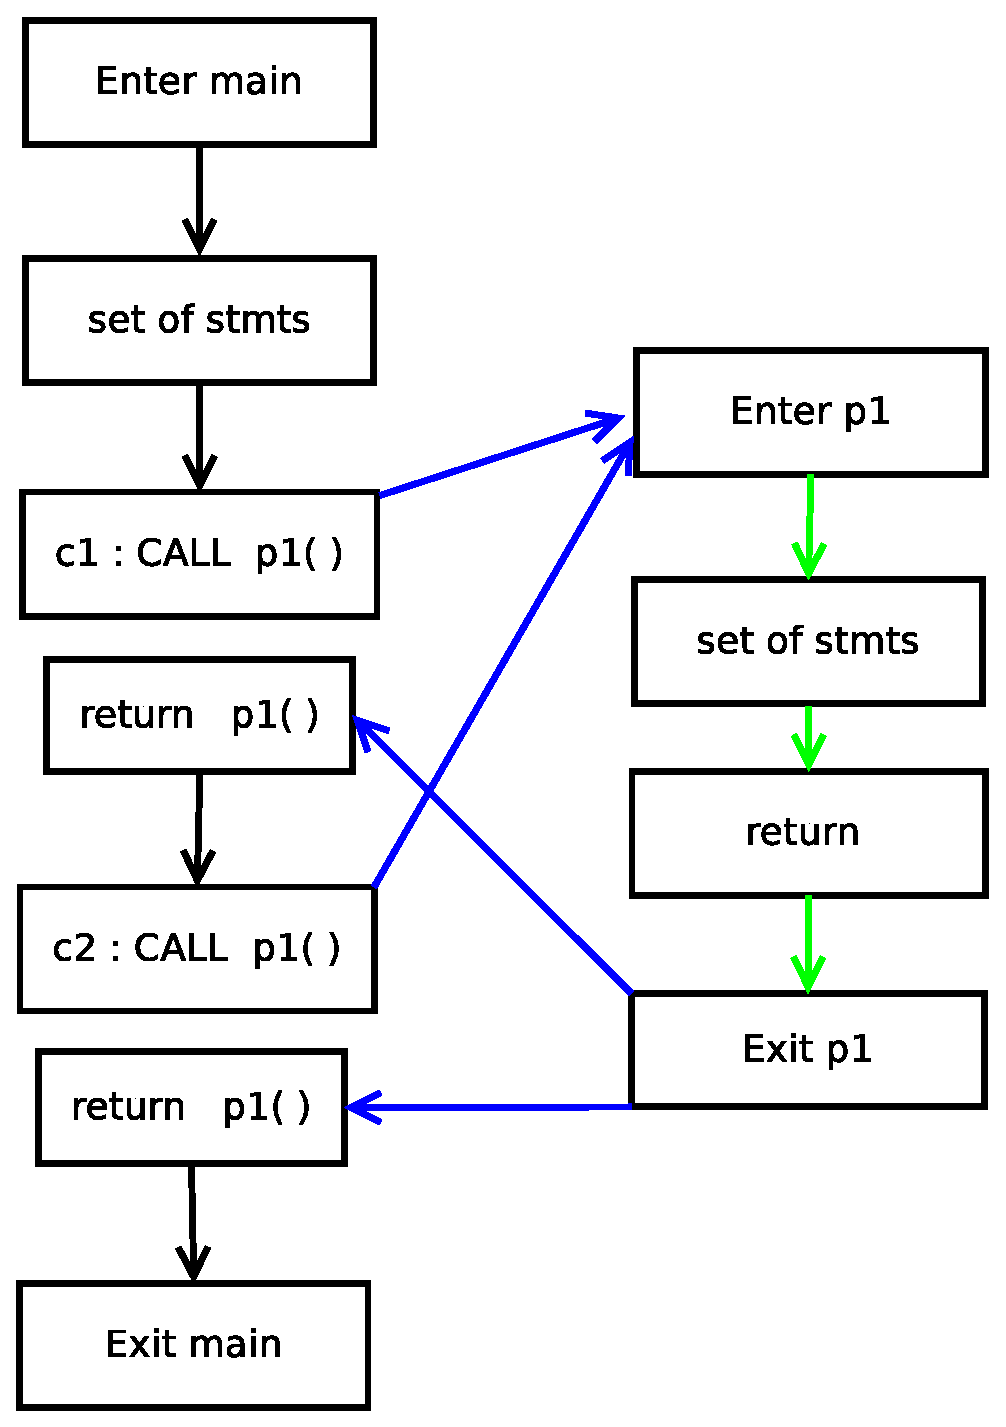
\includegraphics[scale=.23]{Figures/Diagram2.eps} \\
\footnotesize (a)    & \   \   \  \footnotesize (b)
\end{tabular}
\caption{Global control flow graph}
\label{fig:Some}
\end{figure}

\subsubsection{Callstrings Based Approach}
Callstring Method is one of variants of context sensitive interprocedural analysis in which along with the data flow values a 
callstring is also propagated. This method of analysis was proposed by Sharir et .al \cite{TwoApproach}. Callstring at 
any program point means the sequence of unfinished procedure calls reaching that point starting form the main functions entry. This 
new tagged information will make the inter procedural analysis explicit, so at return statements information can be validly propagated.
The data flow information at any program point looks like 
  \begin{center}
$<$ {\tt Call String cs: Data Flow value d} $>$ \\   
  \end{center}
We can notice this representation in Fig.~\ref{fig:Some}(b). Since we know to which call site {\tt df1} or {\tt df2} belongs to, during the 
exit from function {\tt p1}, we can be sure of sending a data flow value to its correct call site. As seen in the figure, {\tt df1'}, {\tt df2'} are 
sent to {\tt c1},{\tt c2} respectively. In this approach only inter procedurally valid paths are used for data flow transfer hence giving more 
precise results. But the problem with this approach is that we have to keep the data-flow values for each callstring
in the memory ,leading to increased memory consumption.

Lets discuss an briefly about the implementation of call string based 
interprocedural Field Sensitive analysis. First we process the Control flow
graph. We create separate basic blocks for call statements and also add a new 
basic block just below call block, i.e.\ the return block.
Then we initialize the global and local worklist's; global worklist contains 
functions and separate local worklist's are present for each function
which holds basic blocks. For handling termination of call string construction 
we use the method proposed in \cite{LazyPointer}.

As mentioned above the memory consumption is more  because we have to maintain 
separate set of data flow values for each callstring. Hence we 
have moved from context sensitive to context insensitive.
Though context insensitive approach takes less memory the accuracy will decrease which is a trade off we have to make.
Later in Subsection~\ref{subsec:Shape_Sensitive_Approach} we will propose ``Shape Sensitive Analysis'', which is a 
middle way approach to the above methods. 
